\chapter{توصیف معماری سیستم}
\noindent
\textbf{
\textit{
تشریح اینترفیس‌های سیستم، کلاک‌ها و نحوهٔ راه‌اندازی سیستم، دیاگرام بلوکی سخت‌افزار، ساختار درختی سیستم و توصیف ماژول‌های سخت‌افزار 
}
}
\pagebreak

\section{ اینترفیس‌های سیستم}
در ابتدا به صورت خلاصه اینترفیس‌های سیستم سخت‌افزاری الگوریتم Skein بیان می‌شود، اینترفیس یک سیستم شامل ورودی‌ها و خروجی‌ها و مشخصات ایشان است. 
\subsection{ورودی‌ها}
ورودی‌ها کد verilog الگوریتم Skein به شرح زیر اند.
\begin{itemize}
\item
\textbf{clk}\\
ورودی کلاک سیستم است که با آن سیستم کار خود را به صورت ترتیبی 
\footnote{\lr{Sequential}}
انجام می‌دهد، فرکانس کلاک با توجه به نحوهٔ پیاده‌سازی سخت‌افزاری و نتایج حاصل از سنتز تعیین می‌شود.
\item
\textbf{\lr{midstate}}\\
ورودی‌ای ۵۱۲ بیتی برای الگوریتم
\lr{Skein-512}
  است که حالت میانی در هش را معلوم می‌کند.
\item
\textbf{nonce}\\
nonce مقداری دلخواه است که برای به حداکثر رساندن تصادفی  و غیرقابل شکستن بودن هش 
در محاسبه هش استفاده می‌شود، این مقدار می‌تواند عددی دلخواه باشد. در الگوریتم 
\lr{Skein-512}
 اندازهٔ این ورودی ۳۲ بیت به اندازه طول عدد در Integer گرفته شده است.
\item
\textbf{data}\\
ورودی اصلی‌ست که باید هش آن محاسبه شود، در کد verilog داده شده اندازه این ورودی ۹۶ بیت در نظر گرفته شده است. 
\end{itemize}

\subsection{خروجی}
تنها خروجی سیستم مقدار هش در output است که ۵۱۲ بیت طول دارد.
(الگوریتم مورد بحث 
\lr{Skein-512}
 است)

\section{کلاک‌ها و نحوهٔ راه‌اندازی سیستم}
این سیستم فقط از یک کلاک استفاده می‌کند و برای راه‌اندازی سیستم انجام کارهای زیر ضروری‌ست.
\begin{enumerate}
\item
وصل کردن کلاک با فرکانس مناسب به سیستم
\item
اعمال ریست‌ کلی بر سیستم
\footnote{\lr{Global Reset}}
\item 
تعیین ورودی‌های اولیه 
\item 
راه‌اندازی سیستم 
\end{enumerate}


\section{دیاگرام بلوکی سخت‌افزار}
دیاگرام بلوکی کلی سخت‌افزار در شکل 
\ref{block_diagram}
آمده است. 

\begin{figure}
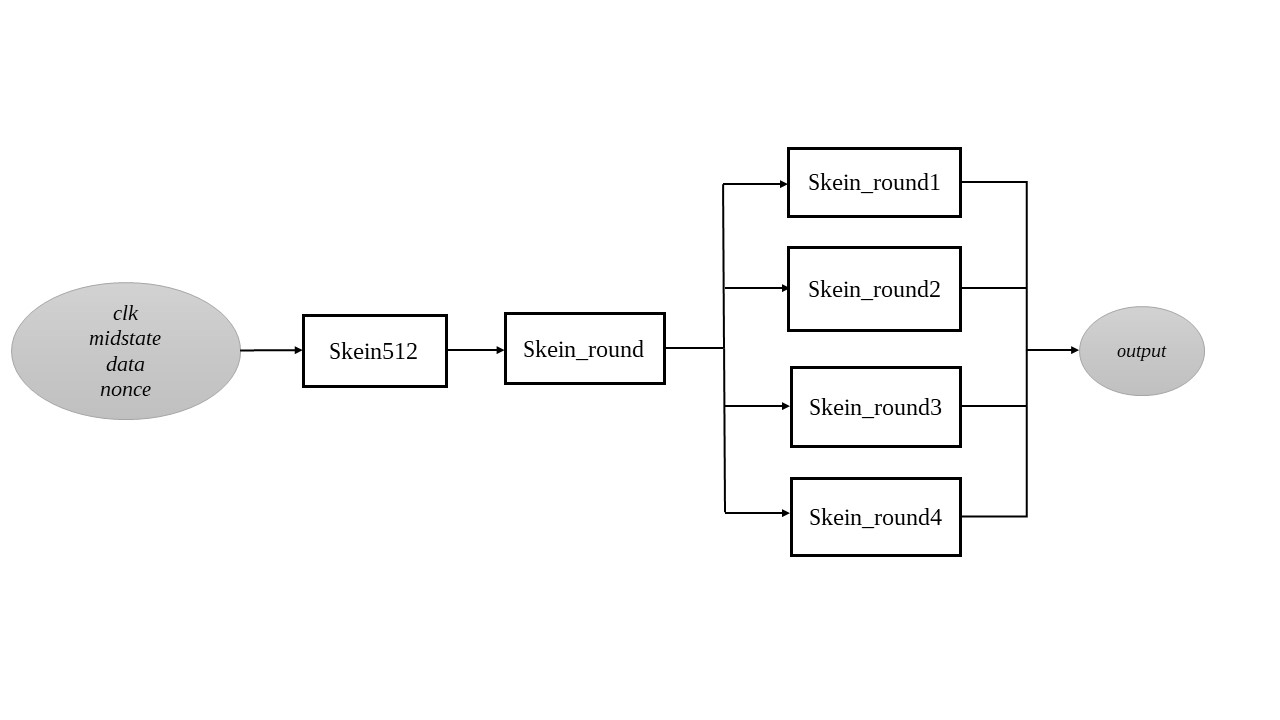
\includegraphics[width = \textwidth]{figs/DescriptionOfSystem/block_diagram.jpg}
\caption{دیاگرام بلوکی سخت‌افزار}
\label{block_diagram}
\end{figure}

\section{توصیف ماژول‌های سخت‌افزار}
\subsection{\lr{Skein-512}}
ابتدا تعدادی reg و wire گرفته شده است.
دو reg به نام های phase\_d و phase\_q تعریف شده اند که یک‌بیتی اند و مقدار صفر به آنها داده شده است.\\
دو عبارت assign در کد وجود دارد.

\begin{enumerate}
	\item در reg 32 بیتی با نام nonce\_le که در خطوط بالاتر تعریف شده است مقادیر nonce (که ورودی 32 بیتی ماژول هستند) به صورت 8 بیت – 8 بیت و به صورت برعکس ذخیره می‌شوند. یعنی به طور مثال 8 بیت کم ارزش\  nonceدر 8 بیت پرارزش nonce\_le ذخیره شده اند. (خط 55)lk\par

	\item در reg 32 بیتی با نام nonce2\_le که در خطوط بالاتر تعریف شده است مقادیر nonce2 (که برعکس nonce، ورودی ماژول نیست و خود در خطوط بالاتر به صورت یک reg 32 بیتی تعریف شده است و در واقع در حال حاضر مقداری را به خود اختصاص نداده است) به صورت 8 بیت – 8 بیت و به صورت برعکس ذخیره می‌شوند. یعنی به طور مثال 8 بیت کم ارزش\  nonce2در 8 بیت پرارزش nonce2\_le ذخیره شده اند. (خط 56)
\end{enumerate}

یک عبارت assign طویل مربوط به hash دیده می‌شود:

\begin{itemize}
\item
در این عبارت بیت‌های reg ی به نام
 h\_q 
که 512 بیت دارد و در خطوط بالاتر تعریف شده است، به بیت های خروجی hash اساین می‌شود.
\item
64 مجموعه 8 بیتی از h\_q به بیت های hash اساین می‌شود که نظم این مقداردهی در زیر توضیح داده می‌شود. در این توضیحات hash را به ترتیب از پرارزش‌ترین بیت شروع به پر کردن میکنیم.
\item
پرارزش‌ترین بیت‌های hash با بیت های 463 تا 456 پر شده است. (یعنی پرارزش ترین بیت hash با بیت 463 ام h\_q پر شده است و به همین ترتیب)
\item
مجموعه بعدی 8 تایی از464 تا 471 هستند که در دومین 8 تایی با ارزش hash قرار می‌گیرند.
\item
این روند تا هشتمین 8 بیت ارزشمند hash ادامه پیدا میکند جایی که در این جایگاه مجموعه [511:504] از h\_q جای میگیرد. (تا اینجا نظم داشتیم)
\item
نهمین 8 بیت ارزشمند hash توسط بیت های [391:384] از h\_q پر میشوند.
\item
این روند ادامه پیدا میکند (یعنی دهمین 8 بیت ارزشمند با [399:392] پر میشوند).
تا 16امین 8 بیت ارزشمند hash که با مجموعه [447:440] پر شده اند.
\item
17امین 8 بیت ارزشمند با مجموعه [327:320] پر میشود.
\item
این روند مانند قبل به صورت صعودی ادامه پیدا خواهد کرد تا به 25 امین مجموعه 8 بیتی برسیم.

\end{itemize}

\textit{\textbf{درواقع هر 8 بار که مجموعه بیت های 8 بیتی را assign میکنیم، یک بی‌نظمی داریم.
}}
\begin{itemize}
\item
25 امین 8 بیتی hash با بیت های [263:256] پر میشود.
\item
دوباره روند سابق و صعودی را داریم تا به 33 امین assignment برسیم.
\item
33 امین 8 بیتی hash با بیت های [199:192]

\end{itemize}

\textit{\textbf{هر بار بی‌نظمی داریم بازه جدید بعد از بی نظمی 120 واحد کمتر از بازه قبلی خواهد بود مثلا 32 امین 8بیت پرارزش hash با بیت های [319:312] پر شده اند که 120 واحد از بازه ای که برای 33امین 8 بیت ارزشمند hash اختصاص داده میشود بیشتر است. (در بالا 33امین نوشته شده است)}}

\begin{itemize}
\item
باز 8 مجموعه که به صورت صعودی پیش برویم به 40 امین 8بیت میرسیم که طبق نظم با بیت های [255:248] پر شده است و 41امین 8 بیتی با بازه [135:128] پر شده است.
\item
باز 8 مجموعه که به صورت صعودی پیش برویم به 48 امین 8بیت میرسیم که طبق نظم با بیت های [191:184] پر شده است و 49امین 8 بیتی با بازه [71:64] پر شده است.
\item
باز 8 مجموعه که به صورت صعودی پیش برویم به 56 امین 8بیت میرسیم که طبق نظم با بیت های [127:120] پر شده است و 57امین 8 بیتی با بازه [7:0] پر شده است.
\item
از 57 امین مجموعه 8 تایی با ارزش hash تا آخرین مجموعه باارزش hash (64 امین) نیز به صورت صعودی و طبق نظم پیش میرود. (خط 121)

\end{itemize}

بعد از خطوط assignment، 18 instance از ماژول skein\_round گرفته شده است.
این instance ها را از 00 تا 0H نام گذاری کردیم (نامگذاری در مبنای بالاتر از 10 شده است)

